\documentclass[12pt]{article}

\usepackage{graphicx}
\usepackage{amsmath}
\usepackage[utf8]{inputenc}  
\usepackage[section]{placeins}
\usepackage{capt-of}
\usepackage{verbatim}
\usepackage{subfig}
\usepackage[a4paper, total={7in, 9.5in}]{geometry}
\usepackage{listings}
\usepackage{color}
\definecolor{mygreen}{RGB}{28,172,0}
\definecolor{mylilas}{RGB}{170,55,241}

\date{}
\title{An Inductorless Step-down Converter Utilizing Inductance of Transmission Cables in Charging Applications}

\author{Circuit Simulation}

\begin{document}
\lstset{language=Matlab,%
    %basicstyle=\color{red},
    breaklines=true,%
    morekeywords={matlab2tikz},
    keywordstyle=\color{blue},%
    morekeywords=[2]{1}, keywordstyle=[2]{\color{black}},
    identifierstyle=\color{black},%
    stringstyle=\color{mylilas},
    commentstyle=\color{mygreen},%
    showstringspaces=false,%without this there will be a symbol in the places where there is a space
    numbers=left,%
    numberstyle={\tiny \color{black}},% size of the numbers
    numbersep=9pt, % this defines how far the numbers are from the text
    emph=[1]{for,end,break},emphstyle=[1]\color{red}, %some words to emphasise
    %emph=[2]{word1,word2}, emphstyle=[2]{style},    
}

\maketitle

\begin{center}
D.K.M.A.M. Padmal - 140427D
\end{center}

\section{Circuit}
The circuit simulations in this report were done with the following circuit created using PLECS\\
\begin{center}
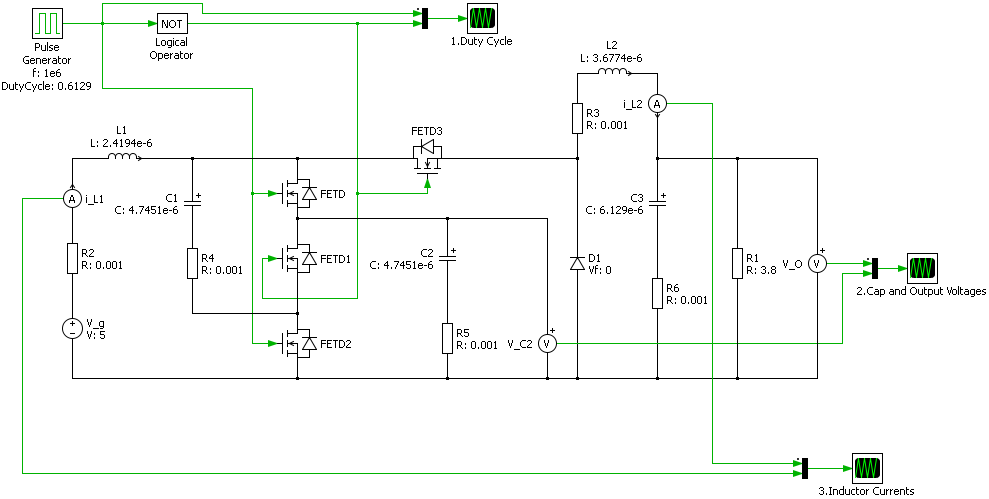
\includegraphics[scale=0.5]{images/schematic.png}
\end{center}

\pagebreak 

\section{Parameters}
Following parameters were used in the circuit simulation

\begin{table}[h]
\centering
\begin{tabular}{| c | c |}
\hline
&\\[-2ex]
\textbf{Component} & \textbf{Simulated Values}\\[0.5ex]
\hline
&\\[-2ex]
Source Voltage ($V_g$) & 5 V\\[0.5ex]
\hline
&\\[-2ex]
Duty Ratio ($D$) & 0.6129\\[0.5ex]
\hline
&\\[-2ex]
Load Resistance ($R_o$) & 3.8 $\Omega$\\[0.5ex]
\hline
&\\[-2ex]
Output Voltage ($V_o$) & 3.8 V\\[0.5ex]
\hline
&\\[-2ex]
Switching Frequency ($f_s$) & 1 MHz\\[0.5ex]
\hline
&\\[-2ex]
Inductor ($L_1$) & 2.4194 $\mu$H, ESR = 0.001$\Omega$\\[0.5ex]
\hline
&\\[-2ex]
Inductor ($L_2$) & 3.6774 $\mu$H, ESR = 0.001$\Omega$\\[0.5ex]
\hline
&\\[-2ex]
Capacitor ($C_1$, $C_2$) & 4.7451 $\mu$F, ESR = 0.001$\Omega$\\[0.5ex]
\hline
&\\[-2ex]
Capacitor ($C_o$) & 6.1290 $\mu$F, ESR = 0.001$\Omega$\\[0.5ex]
\hline
\end{tabular}
\end{table}


\section{Simulations}
\subsection{Duty Cycle}
Pulse generator is used to generate the square wave to drive the MOSFETs and the following waveform is observed.

\begin{center}
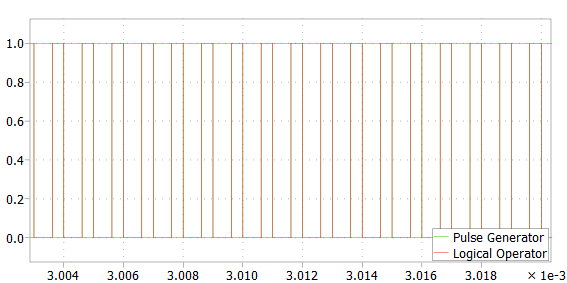
\includegraphics[scale=0.8]{images/duty_graph.png}
\end{center}

\pagebreak 
\subsection{Output Voltage Waveforms}
Output voltage waveform is observed across the $R_o$ resistor and an intermediate waveform can be observed across the $C_1$ or $C_2$ capacitor.

\begin{figure}[h]
\caption{Output Voltage Waveform}
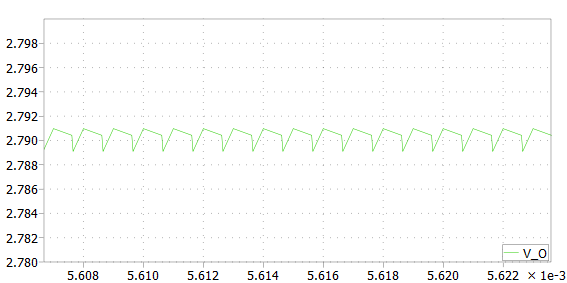
\includegraphics[scale=0.8]{images/v_o_graph.png}
\end{figure}

\begin{figure}[h]
\caption{Capacitor Voltage Waveform}
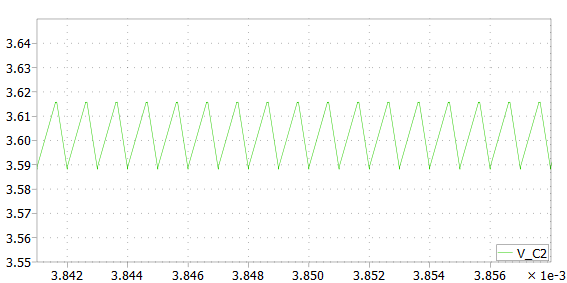
\includegraphics[scale=0.8]{images/v_c_graph.png}
\end{figure}

\pagebreak 
\subsection{Inductor Current Waveforms}
Current across the inductors $L_1$ and $L_2$ were observed as follows;

\begin{figure}[h]
\caption{Inductor Current Waveforms}
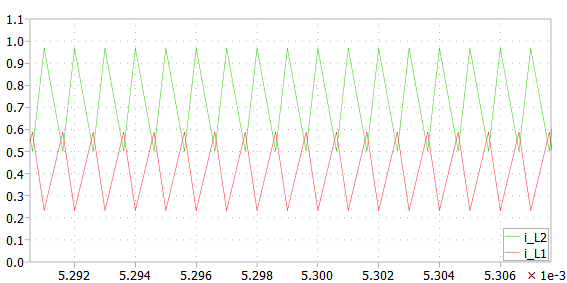
\includegraphics[scale=0.8]{images/i_l_graph.png}
\end{figure}

\section{Voltage Gain}

Output voltage expression was derived as follows;
\begin{equation*}
V_o = \frac{2DV_g-(1+D)V_{D_1}D'}{(1+D)+\frac{R_Z}{R_o}}
\end{equation*}\\
By dividing both sides by $V_g$ we can derive the voltage gain function for non ideal case.
\begin{equation*}
\frac{V_o}{V_g} = \frac{2D-(1+D)\frac{V_{D_1}}{V_g}D'}{(1+D)+\frac{R_Z}{R_o}}
\end{equation*}\\
This will simplify into;
\begin{equation*}
M = \frac{2D}{(1+D)+\frac{R_Z}{R_o}} - \frac{(1+D)\frac{V_{D_1}}{V_g}D'}{(1+D)+\frac{R_Z}{R_o}}
\end{equation*}\\
There is another step taken in the plots. That is when the diode forward voltage is zero and when it is 0.6 V.
\\

For both ideal and non-ideal cases, gain function can be plotted as follows;

\begin{figure}[!h]
\caption{Gain Plots when $V_f$ = 0 V}
\centering
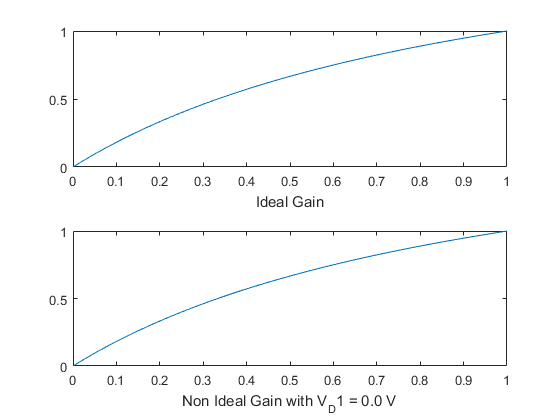
\includegraphics[scale=0.8]{images/gain_ovd.png}
\end{figure}

\begin{figure}[!h]
\caption{Gain Plots when $V_f$ = 0.6 V}
\centering
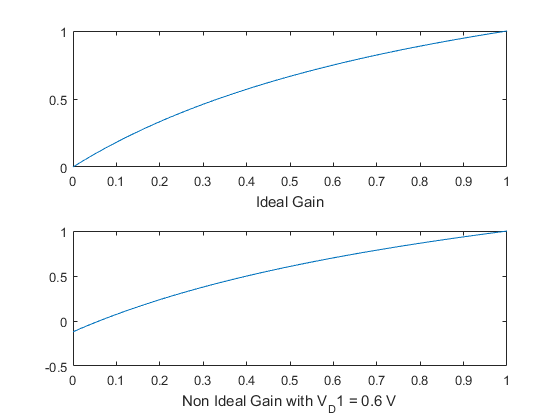
\includegraphics[scale=0.8]{images/gain_wvd.png}
\end{figure}

\section{Transfer Functions}
There are two transfer functions taken into consideration at four different input parameters.

\subsection{Line to Output Transfer Function}
Line to Output transfer function ($G_{vg}(s)$) is expressed as;
$$G_{vg}(s) = \frac{(1+D)}{2D}\frac{u(s)}{z(s)}$$
Where;
$$z(s) = \frac{R_o + (L_a + L_2)s + (L_a C_o + L_a C_a + L_2 C_o)R_o s^2 + L_a L_2 C_a s^3 + L_a C_a L_2 C_o R_o s^4}{1+R(C_a + C_o)+L_2 Cs^2 + L_2 C_o CR_o S^3}$$
$$u(s) = \frac{R_o}{1+R_o C_o s}$$
$$L_a = \frac{4D^2}{(1+D)^2}L_1$$
$$C_a = \frac{C}{D^2}$$

\begin{figure}[h]
    \centering
    \subfloat[$G_{vg}(s)$ when $V_o = 3.3 V$ and $I_o = 1 A$]{{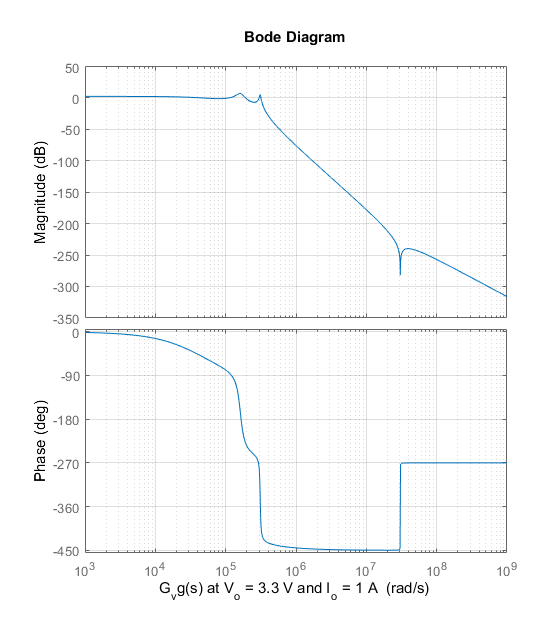
\includegraphics[width=8cm]{images/gvg1.png} }}%
    \qquad
    \subfloat[$G_{vg}(s)$ when $V_o = 3.8 V$ and $I_o = 1 A$]{{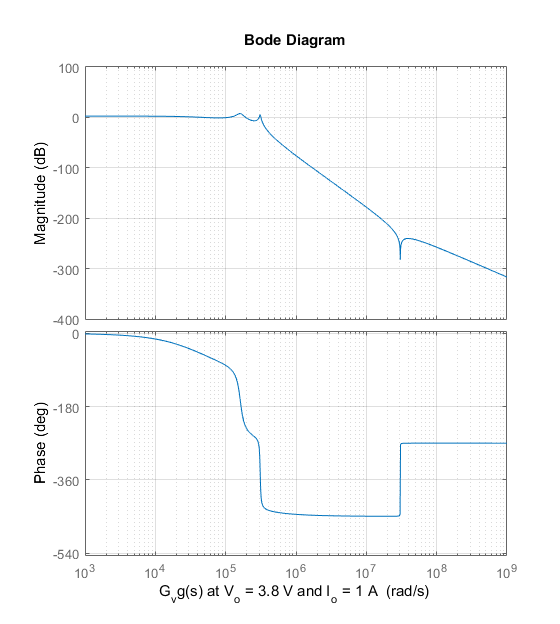
\includegraphics[width=8cm]{images/gvg2.png} }}%
    \qquad
    \subfloat[$G_{vg}(s)$ when $V_o = 4.2 V$ and $I_o = 1 A$]{{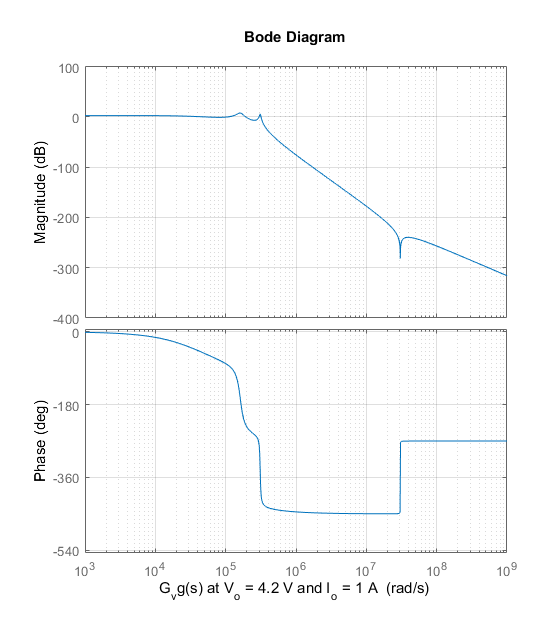
\includegraphics[width=8cm]{images/gvg3.png} }}%
    \qquad
    \subfloat[$G_{vg}(s)$ when $V_o = 4.2 V$ and $I_o = 0.5 A$]{{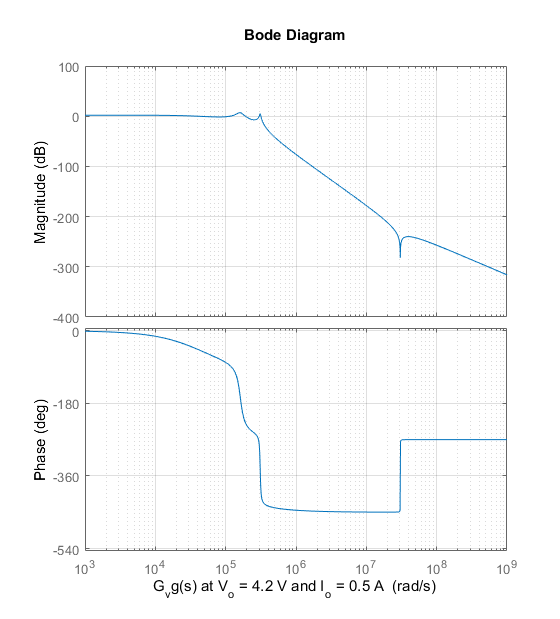
\includegraphics[width=8cm]{images/gvg4.png} }}
\end{figure}

\pagebreak

\subsection{Control to Output Transfer Function}
Control to Output transfer function ($G_{vd}(s)$) is expressed as;

$$G_{vd}(s) = e(s)\frac{(1+D)}{2D}\frac{u(s)}{z(s)}$$
Where;
$$z(s) = \frac{R_o + (L_a + L_2)s + (L_a C_o + L_a C_a + L_2 C_o)R_o s^2 + L_a L_2 C_a s^3 + L_a C_a L_2 C_o R_o s^4}{1+R(C_a + C_o)+L_2 Cs^2 + L_2 C_o CR_o S^3}$$
$$u(s) = \frac{R_o}{1+R_o C_o s}$$
$$L_a = \frac{4D^2}{(1+D)^2}L_1$$
$$C_a = \frac{C}{D^2}$$

\begin{figure}[h]
    \centering
    \subfloat[$G_{vd}(s)$ when $V_o = 3.3 V$ and $I_o = 1 A$]{{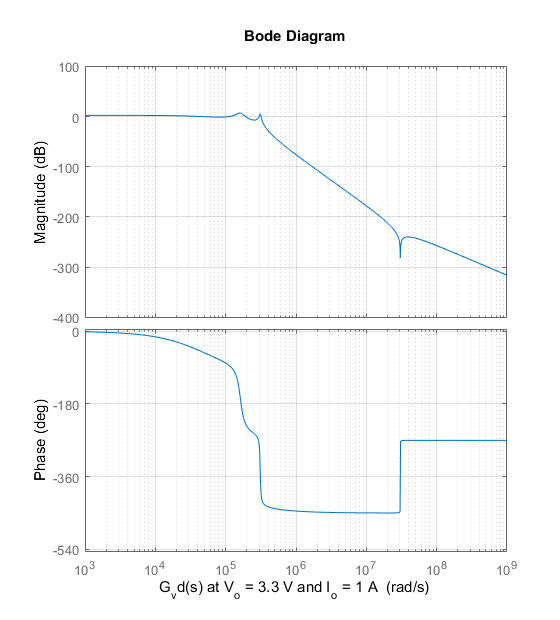
\includegraphics[width=8cm]{images/gvd1.png} }}%
    \qquad
    \subfloat[$G_{vd}(s)$ when $V_o = 3.8 V$ and $I_o = 1 A$]{{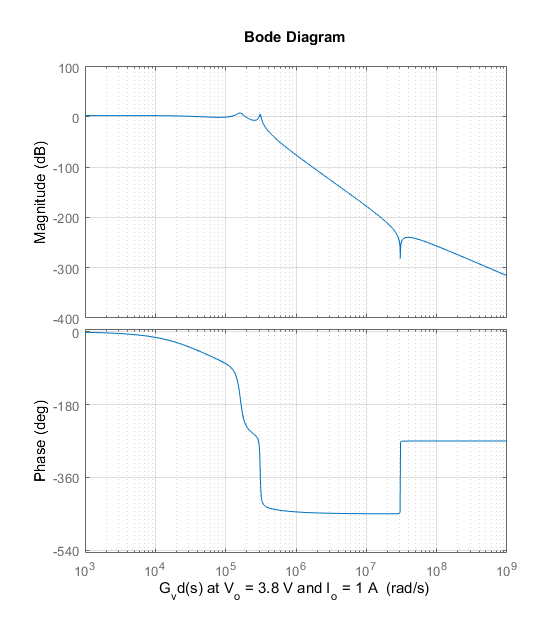
\includegraphics[width=8cm]{images/gvd2.png} }}%
    \qquad
    \subfloat[$G_{vd}(s)$ when $V_o = 4.2 V$ and $I_o = 1 A$]{{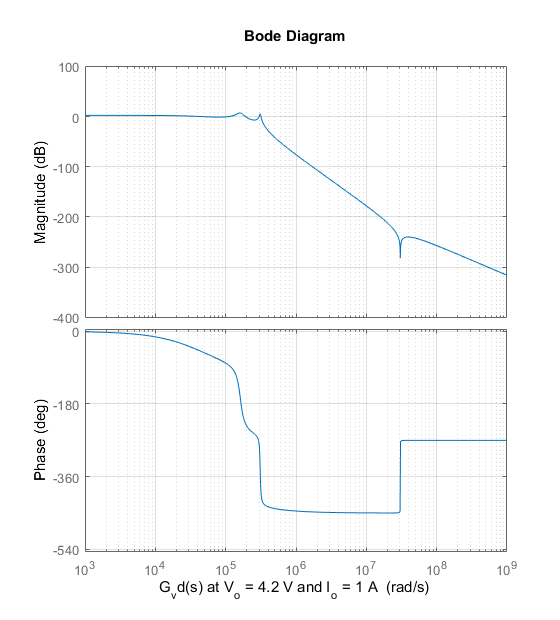
\includegraphics[width=8cm]{images/gvd3.png} }}%
    \qquad
    \subfloat[$G_{vd}(s)$ when $V_o = 4.2 V$ and $I_o = 0.5 A$]{{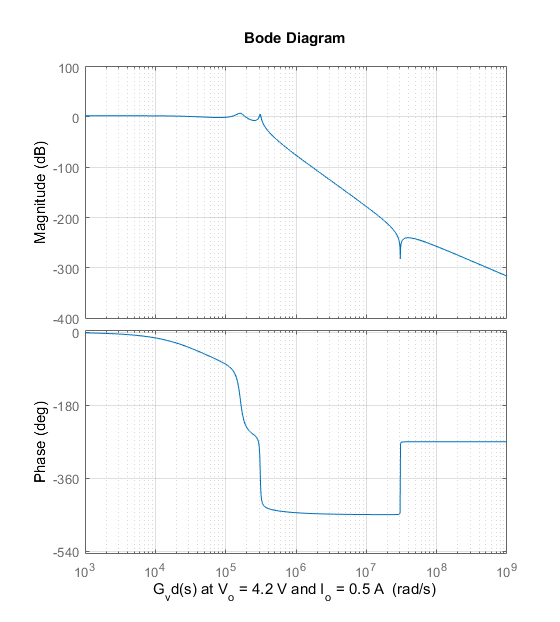
\includegraphics[width=8cm]{images/gvd4.png} }}%
\end{figure}

\pagebreak
\subsection{Source Code}

\subsubsection{Gain Plots}

\lstinputlisting{images/GainM.m}

\bigskip 
\subsubsection{Transfer Functions}

\lstinputlisting{images/TFsM.m}

\end{document}